\documentclass[12pt]{article}
\usepackage[top=1in, bottom=1in, left=1in, right=1in]{geometry}
\usepackage[justification=centering]{caption}
\usepackage{graphicx}
\usepackage{listings}
\usepackage{color}
\usepackage{indentfirst}
\usepackage{hyperref}
\usepackage{siunitx}
\usepackage{float}
\usepackage{amsmath}

\lstset{ %
	%language=C,                % choose the language of the code
	basicstyle=\scriptsize,       % the size of the fonts that are used for the code
	                  % how far the line-numbers are from the code
	backgroundcolor=\color{white},  % choose the background color. You must add \usepackage{color}
	showspaces=false,               % show spaces adding particular underscores
	showstringspaces=false,         % underline spaces within strings
	showtabs=false,                 % show tabs within strings adding particular underscores
	%frame=single,           % adds a frame around the code
	tabsize=2,          % sets default tabsize to 2 spaces
	captionpos=b,           % sets the caption-position to bottom
	breaklines=true,        % sets automatic line breaking
	breakatwhitespace=false,    % sets if automatic breaks should only happen at whitespace
	escapeinside={\%*}{*)}          % if you want to add a comment within your code
}

\begin{document}
\title{Microprocessor Systems\\ Lab 6: Memory Interfacing }
\author{Alvin Chia \and Nick Choi \and Samuel Deslandes \and Shanmugam Thiagarajan}
\date{12/13/16}
\maketitle
\pagebreak
\section{Introduction}



\section{Methods}
\subsection{Software}
The program for this project was organized into several functions. The `main()' function handles initializations and repeatedly calls the `playGame()' function on an infinite loop. `playGame()' handles the main game play operations such as the main menu, moving the cursor, keeping track of time and score and displaying them on the LCD screen, and checking win and lose game states. Other functions such as `drawTarget()', `checkTarget()', and `eraseTarget()' handle the display and hit detection aspects of targets. 

\subsubsection{Main() and Configurations}
`Main()' begins by disabling the watchdog timer and calling the various initialization functions. In `PORT\_INIT()' the crossbar is configured such that UART0 is enabled in the `XBR0' SFR, /INT0 and /INT1 are routed to port pins in `XBR1', and in 'XBR2' the crossbar is enabled with weak pull-up. Next global interrupts and external interrupt 1 is enabled using the bit addressable keywords `EA' and `EX1', respectively. /INT1 associated with the button on the joystick is also set to be triggered on falling edge by setting `IT1` to 1. Lastly the ports are configured. P0.0 and P2.0 are set for push-pull operation for use by TX and a buzzer respectively. Port3 is used by the keypad, and is configured such that its high nibble in push-pull mode with digital LO output, and its low nibble is in open-drain mode with high impedance. 

`SYSCLK\_INIT()' initializes the system clock to use just the external oscillator with a frequency of 11.0592\si{Mhz}. In `UART0\_INIT()' Timer1 is used to generate a baud rate 115200. To accomplish this Timer1 is configured using the `TMOD' SFR to be an 8-bit counter with auto-reload. The auto-reload value for the required baud rate is \texttt{0xFA}. A reference reload values for each timer, SYSCLK, and desired baud rate can be found on page 295 of the C8051 manual[3]. The UART itself is configured to be in mode 1 using the `SCON0' SFR. In 'ADC0\_INIT()', `ADC0CF' is set to \texttt{0xBF}, resulting in a gain term of $\frac{1}{2}$, and a SARclk of 230400\si{Hz}. The can be calculated as follows: 
\begin{gather*}
ADC0SC=\frac{SYSCLK}{2\times SARclk}-1\\
\textrm{where ADC0SC is bits 3--7 of ADC0CF}
\end{gather*}
The internal reference buffer and bias generator are enabled, producing a voltage of 2.4\si{V}, which is used as a reference for conversions. 

Finally, Timer0 is used to accurately count game time in measurements of a tenth of a second. It's configured as a 16-bit counter using SYSCLK/48 as a base. For an overflow of this timer to occur every tenth of a second, the timer must be set to start counting at \texttt{0xA600} on initialization as well as after every overflow. This can be calculated as follows:
\begin{gather*}
\frac{1}{48}\times \frac{11059200 \si{counts}}{\si{1}{sec}}=\frac{X\si{counts}}{0.1\si{sec}}
\end{gather*}
Solving for $X$ gives $X=23040$. Since 23040 counts elapse in a tenth of a second, the timer must start counting from $2^{16}-23040=42496$. This corresponds to \texttt{0xA600} in hex. Since Timer0 is a 16-bit counter, this must be split between its high and low registers, with $\mathrm{TH0}=\texttt{0xA6}$ and $\mathrm{TL0}=\texttt{0x00}$.

\subsubsection{playGame()}


\subsubsection{Target handling}


\subsection{Hardware}



\section{Results}

\section{Conclusion}
 


\section{Appendices}
\subsection{Code}
	\lstinputlisting{main.c}
\subsection{Schematics}
\begin{figure}[H]
	\centering
	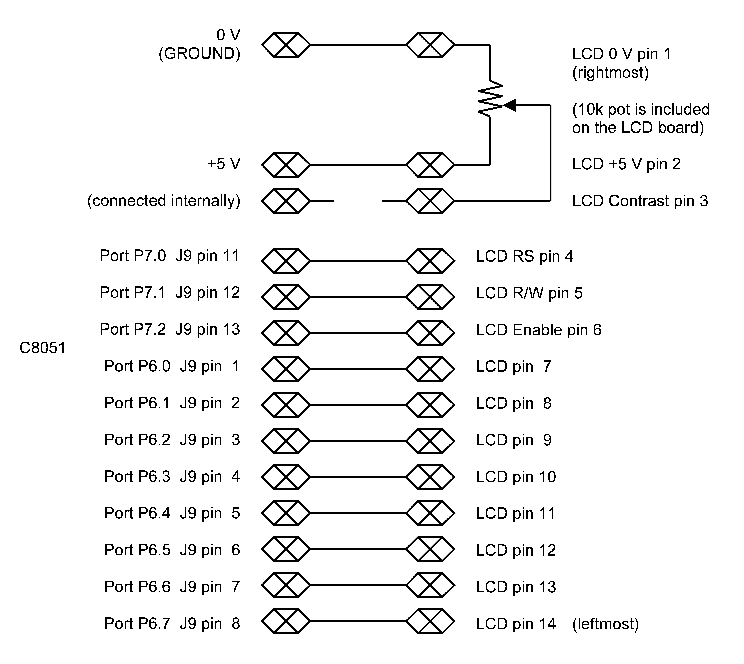
\includegraphics[width=\textwidth]{lcd_schematic.png}
	\caption[]{Circuit schematic for LCD[2]}
	\label{LCD}
\end{figure}


\section{References} 
\noindent
[1]``MPS Lab 6," in RPI ECSE Department, 2016. [Online]. Available: \url{http://www.rpi.edu/dept/ecse/mps/MPS_Lab_Ex6-Magic8Ball.pdf}. Accessed: Nov. 27, 2016.\\
\newline\noindent
[2]``Interfacing a Hitachi HD44780 to a Silicon Laboratories C8051F120," in RPI ECSE Department, 2016. [Online]. Available: \url{http://www.rpi.edu/dept/ecse/mps/LCD_Screen-8051.pdf}. Accessed: Nov. 27, 2016.\\
\newline\noindent
[3]``C8051 Manual," in RPI ECSE Department, 1.4 ed., 2005. [Online]. Available: \url{https://www.ecse.rpi.edu/courses/CStudio/Silabs/C8051F12x-13x.pdf}. Accessed: Nov. 27, 2016.


\end{document}